\chapter{\textbf{Introdução}}
\label{Introducao}
O projeto ProInfoData tem como objetivo monitorar diariamente os computadores de
todas as escolas públicas do Brasil. O monitoramento visa disponibilizar dados
para que o MEC e a sociedade acompanhem o estado de funcionamento dos
computadores. Inicialmente este parque computacional foi estimado em 500.000
computadores, atualmente, essa estimativa aumentou para mais de 1.000.000 de
máquinas, e a tendência é que continue crescendo com o tempo.
 
Para atender esta demanda de máquinas o sistema foi estruturado da
seguinte forma: todo computador de escola pública brasileira terá um agente (cliente)
que diariamente envia informações de uso e de hardware para o servidor central,
além das informações do uso de rede que foram incluídas recentemente. O servidor
tem duas camadas: o WebService que recebe informações dos agentes e as armazena
no Banco de Dados (BD). Essa arquitetura pode ser visualizada na figura \ref{arquiteturaBD}
seguir:\newline

\begin{figure}[ht]
  \centering
  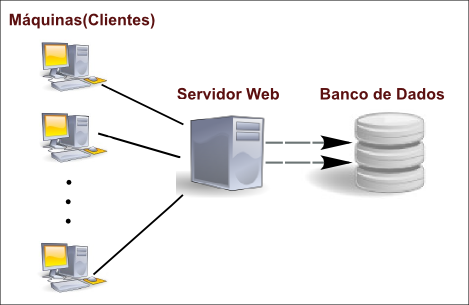
\includegraphics[width=200px,height=150px]{img/arq-bd.png}
  \caption{Visão geral da Arquitetura do ProInfoData}
  \label{arquiteturaBD}
\end{figure}

Como Sistema de Gerenciamento de Banco de Dados (SGBD) foi escolhido um SGBD
relacional. Um dos motivos para essa escolha é porque o modelo relacional facilita
a associação dos dados. Para comportar o volume de dados gerado foi necessário
desenvolver uma arquitetura de armazenamento robusta e escalável. A arquitetura
proposta foi baseada em armazém de dados (Data Warehouse - DW) que é direcionada
às operações de leitura, favorecendo a análise de grandes volumes de dados e a
geração de relatórios complexos, entraremos em mais detalhes no capítulo 2.

No entanto, com o aumento emergente do número de máquinas e com o acréscimo das
informações do uso de rede, o volume de dados tornou-se extremamente grande, fato que 
nos levou a propor um nova solução para o armazenamento dos dados e para realização
das consultas disponíveis no portal do projeto\footnote {\href {http://seed.c3sl.ufpr.br/seed/attendance/index.html}
{portal do projeto}}.

A solução que proposmos baseia-se em uma tecnologia emergente, chamada MapReduce.
Essa solução mostrou-se eficiente em diversas implementações, a mais conhecida é
o sistema de armazenamento e busca do Google \cite{MapReduceGoogle} \footnote{\href {http://labs.google.com/papers/mapreduce.html} {http://labs.google.com/papers/mapreduce.html}}.

Acreditamos que o grande desafio dessa solução será a transformação do modelo
relacional para um modelo "chave-valor".

No capítulo 2 descrevemos com mais detalhes o conceito de Data Warehouse e a arquitetura
do projeto ProInfoData. No capítulo 3 descrevemos o conceito de MapReduce, as 
tecnologias que serão utilizadas, como Hive e Hadoop, e porque utlizar MapReduce no 
ProInfoData. No capítulo 4 nos deparamos com nosso grande desafio em propor um método de 
transformação de Data Warehouse para MapReduce. Enfim, no capítulo 5 chegamos as
conclusões dessa monografia.